\chapter{Tracker}
\label{cha:tracker}

The previous sections have shown how a node can initialize a connection to another node using the EasyRTC Framework: at the beginning they both have to contact the EasyRTC Server to obtain the ID, and then pass the identifier of the other node to the \textit{connect} function in order to establish the connection. However, EasyRTC does not specify how the nodes have to exchange these identifiers: for this purpose we created a tracker. 

When the nodes bootstrap, they have to contact the EasyRTC Server in order to join the network and then they have to register themselves to the tracker. In this way the latter will eventually have the complete list of the nodes present in the network. When a peer needs to connect to another one (i.e. to replace a broken link):
\begin{itemize}
	\item it asks the tracker a reference of a new node
	\item the tracker chooses an ID at random from the list and it returns it to the peer
	\item the peer analyzes the answer and connects to that ID
\end{itemize}

We use the tracker to provide all nodes with a list of ``initial peers'' to contact in order to start the algorithm (more information in Sect.\ref{cha:wormhole}), to replace the broken links and for all the necessary replacements expected from the algorithm. The main tasks of the tracker are shown in Fig. \ref{fig:tracker}.

In this project the tracker acts like a central server: we only have one tracker for all the nodes, and it has to handle and serve all the requests that derive from the nodes. However, this is not a problem since it has relatively low load (the link replacements are rare) and the algorithm is designed to reduce the number of new network connections created. 

The tracker is hosted on Heroku\footnote{Heroku is a cloud platform that lets companies build, deliver, monitor and scale apps \url{https://www.heroku.com/}} and is implemented in \textit{Node.js}. The nodes contact the tracker using \texttt{XMLHttpRequest} (XHR)\footnote{\texttt{XMLHttpRequest} is an API available to web browser scripting languages such as JavaScript that is used to send HTTP or HTTPS requests to a web server and load the server response data back into the script} and then they parse the response to obtain what they asked.

\begin{figure}[ht]
  \centering
  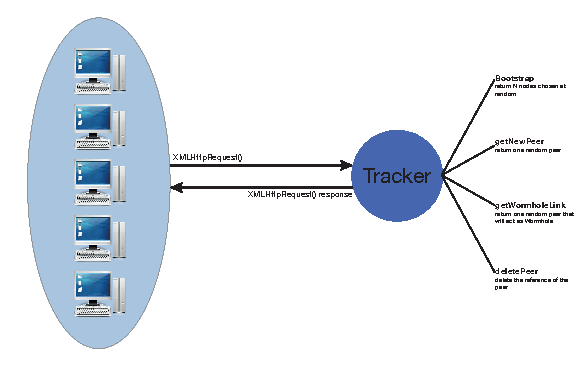
\includegraphics[keepaspectratio=true, width=\textwidth]{images/tracker}\caption{The main tasks of the tracker}
  \label{fig:tracker}
\end{figure}
